\subsubsection{Simulering af kamera}
Til at generere et billedsæt, der simulerer langerhanske øer, er der udviklet et Matlab script. Scriptet består overordnet af 3 faser. Den første fase består i at segmentere langerhanske øer udfra et billede og oprette dem som en maske. I anden fase laves en maske bestående af ekstra væv, mens der i tredje fase simuleres flow. I den sidste fase gemmes også de enkelte billeder i formatet .png (Portable Network Graphic). De enkelte faser er nærmere beskrevet under deres afsnit. Der anvendes 3 billeder til grundlag for generingen. Det ene billede viser isolerede øer. Det andet billede viser opløsningen indeholdende øer og ekstra væv. Det sidste billede er et baggrundsbillede uden øer eller ekstra væv. Dette billede anvendes til baggrunden til de genererede billeder. De 3 billeder er herunder vist.

\begin{figure}[htbp] \centering
\begin{minipage}[b]{0.3\textwidth} \centering
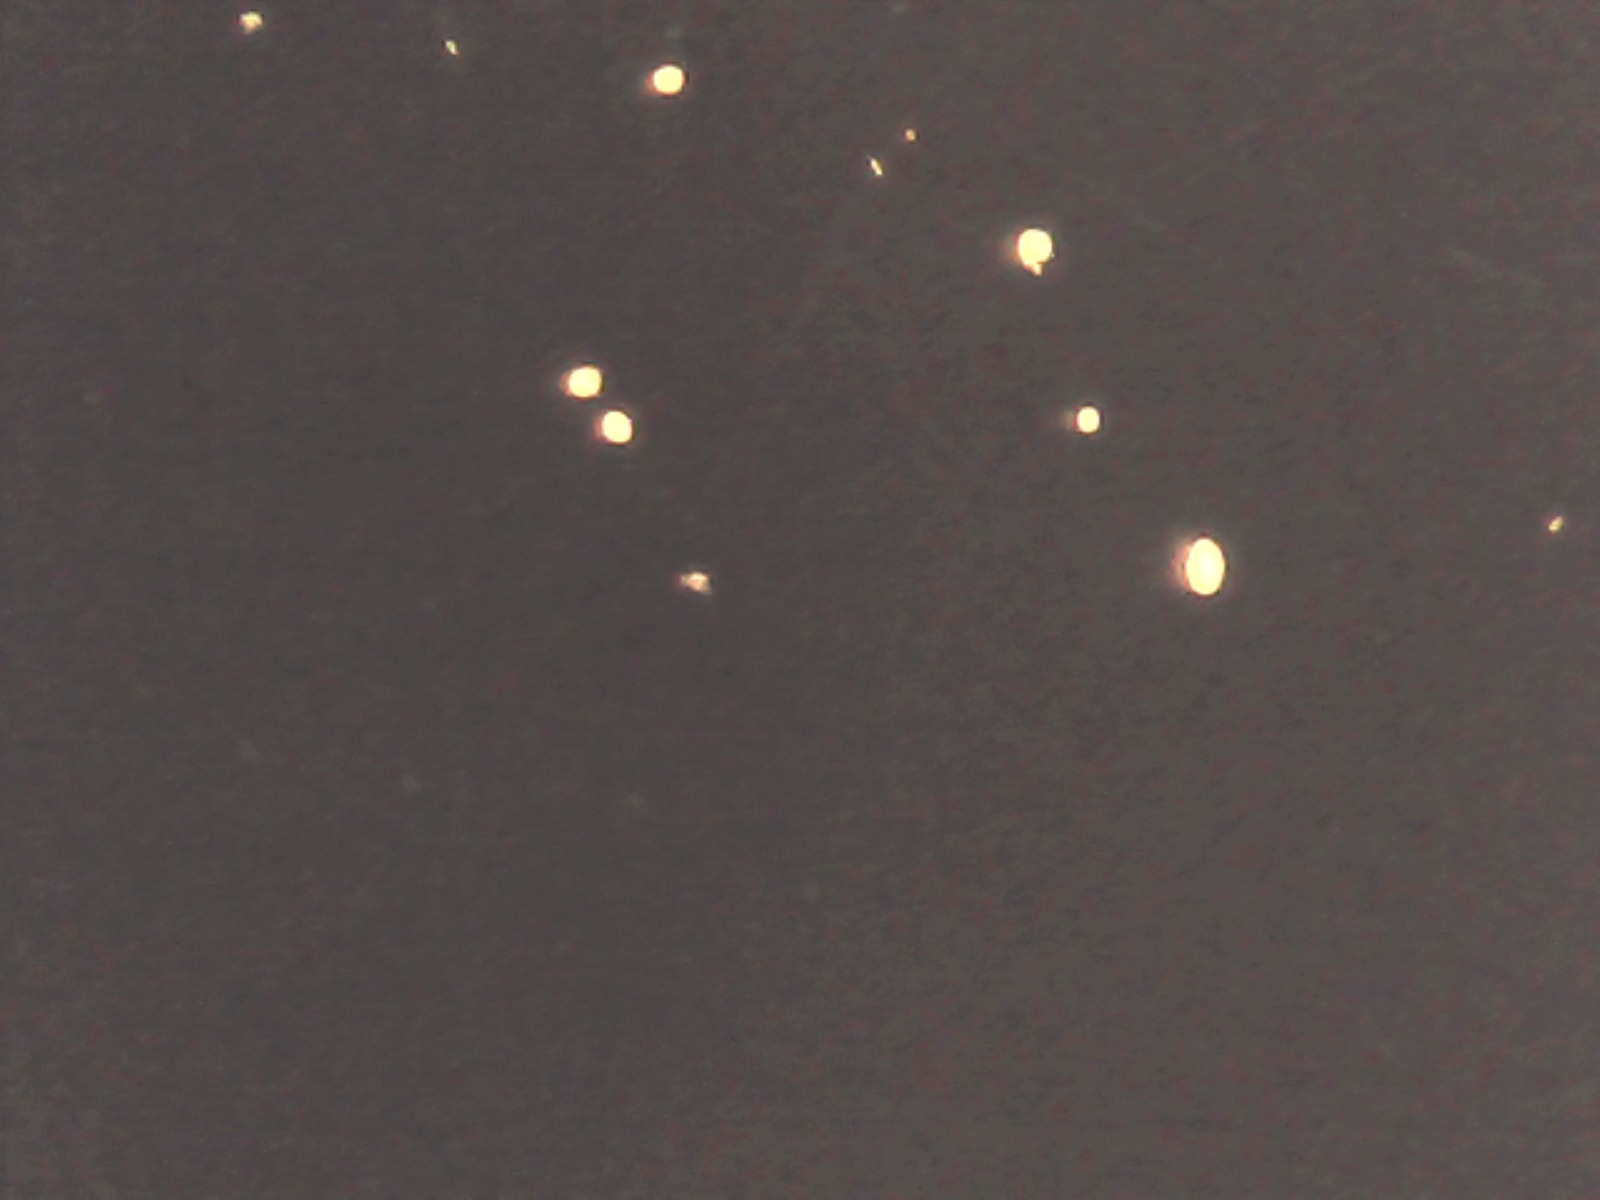
\includegraphics[width=1.00\textwidth]{billeder/software/1.jpg} % Left picture
\end{minipage} \hfill
\begin{minipage}[b]{0.3\textwidth} \centering
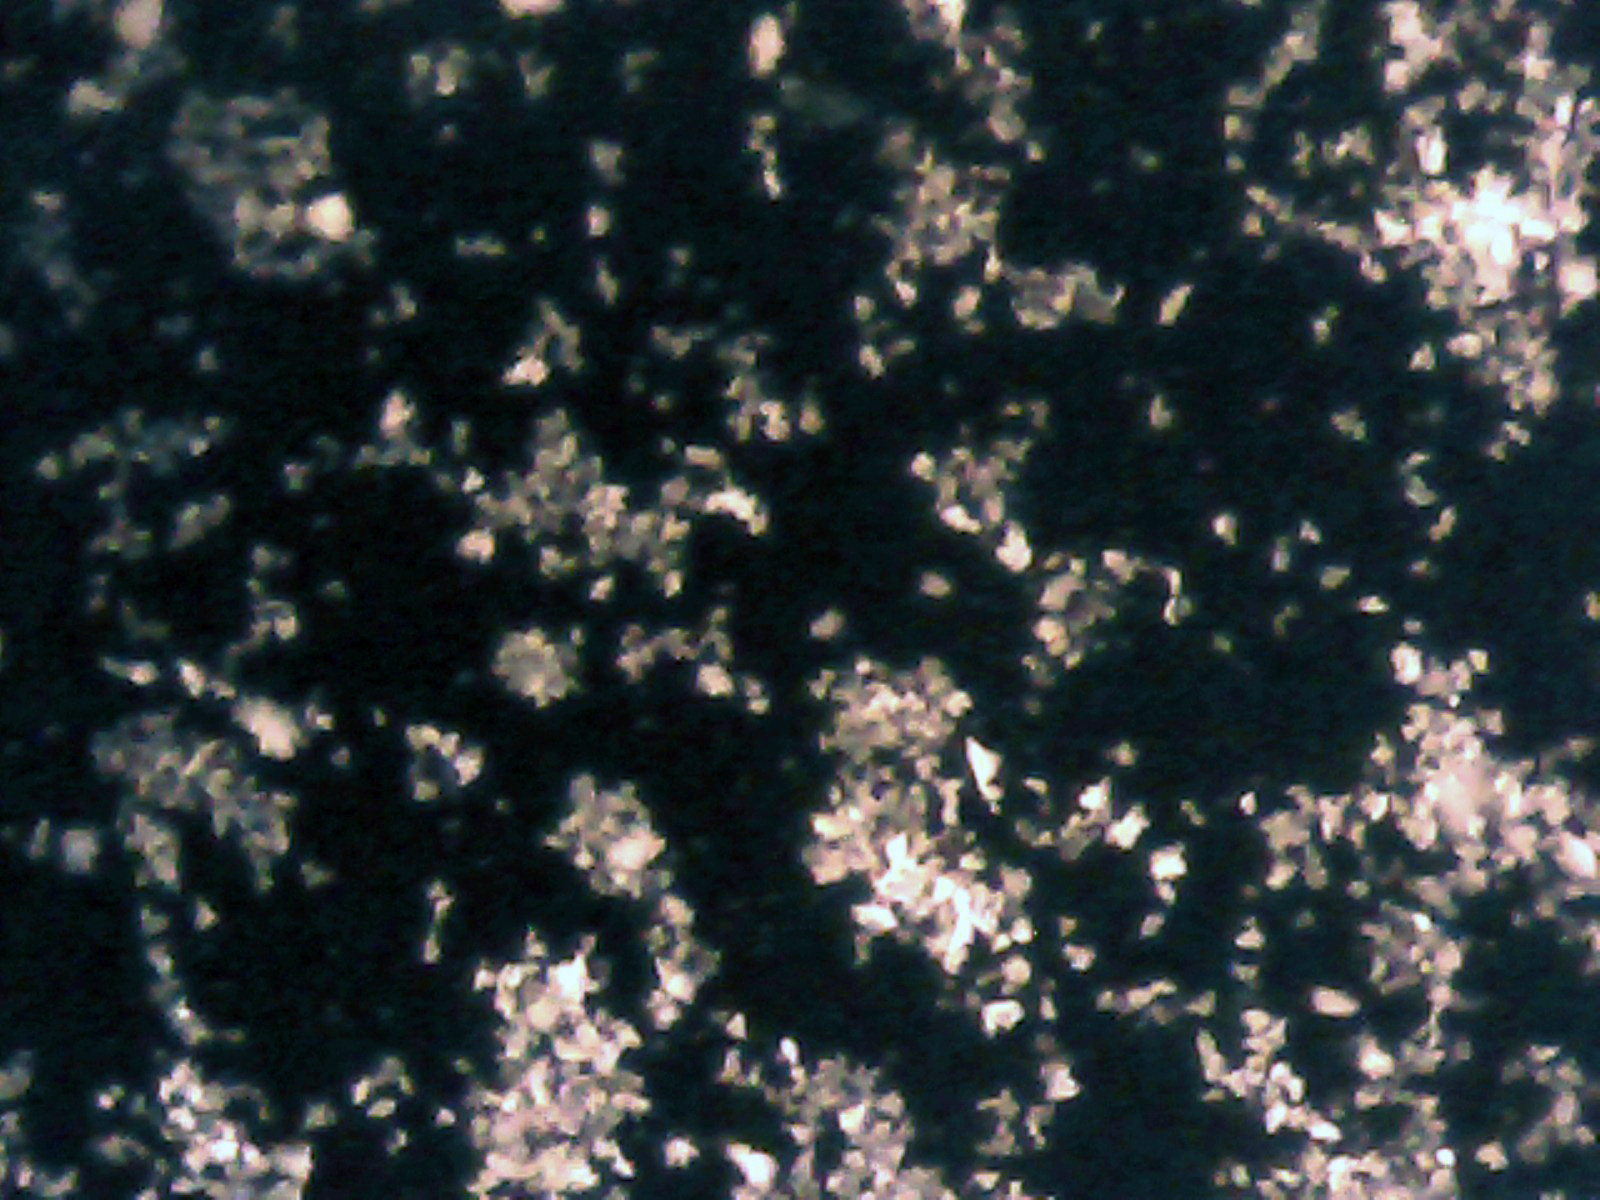
\includegraphics[width=1.00\textwidth]{billeder/software/2.jpg} % Right picture
\end{minipage} 
\hfill
\begin{minipage}[b]{0.3\textwidth} \centering

\includegraphics[width=1.00\textwidth]{billeder/software/3.jpg} % Right picture
\end{minipage} \\  % Captions og labels
\begin{minipage}[t]{0.3\textwidth}
\caption{Billede indeholdende langerhanske øer} % Left caption and label
\label{fig:img1}
\end{minipage} \hfill
\begin{minipage}[t]{0.3\textwidth}
\caption{Billede indeholdende ekstra væv} % Right caption and label
\label{fig:img2}
\end{minipage}
\hfill
\begin{minipage}[t]{0.3\textwidth}
\caption{Baggrundsbillede} % Right caption and label
\label{fig:img3}
\end{minipage}
\end{figure}

\textbf{Fase 1}

Segmenteringen af langerhanske øer sker ud fra billede 1 \ref{fig:img1}, hvor funktionen circleFinder anvendes til at finde centrum og radius på af de fundne celler. 

\textbf{Fase 2}

I anden fase bliver det ekstra væv segmentet ud fra billede 2 (REF). Til dette er der anvendt Color Threshold appen i Matlab. Ved hjælp af denne app er der lavet en funktion, som opretter en logisk maske af det ekstra væv. Opsætningen i appen er vist i figur (REF) \fxnote {Indsæt figur}. Yderligere er der anvendt morfologiske operationer til at fjerne uønskede objekter fra masken, samt fjerne støj. Til at fjerne uønskede objekter er funktionen bwareafilt anvendt, med parametrene 150 og 500. Dette fjerner alle objekter under 150 og over 500 sammenhørende pixels. Til at udfylde huller i de enkelte objekter er funktionen imfill brugt. 

\textbf{Fase 3}

I fase 3 sker selve flow simuleringen. Flowsimuleringen er opbygget på den måde, at den består af henholdvis en sekvens indeholdende en langerhansk ø efterfulgt af en sekvens uden en ø. I selve programmet indlæses et nyt billede hvert 0,1 sekund. Derfor skal der generes en passende mængde billeder, som programmet kan indlæse. Fase 3 er implementeret så der minimum genereres 252 eller maksimalt 432 billeder, hvilket giver en samlet sekvenslængde på 25,2 eller 43,2 sekund. Grunden til at antallet af billeder varierer er at længden af sekvensen uden en langerhansk ø bestemmes udfra en random variabel. I scriptet genereres der i alt 18 sekvenser. Det betyder, at der passerer i mellem 25 og 43 øer i minuttet.
\begin{align}
\frac{18}{n/10} * 60 = \text{Antal øer pr. minut}
\end{align}
I figur \ref{fig:boxplot} er vist et boxplot som viser distributionen af hvor mange øer der passere i minuttet. Det ses at medianen ligger over 30 øer pr. minut, hvilket betyder at der i gennemsnit vil komme over 30 øer pr minut.

 \begin{figure}[H]
	\centering
	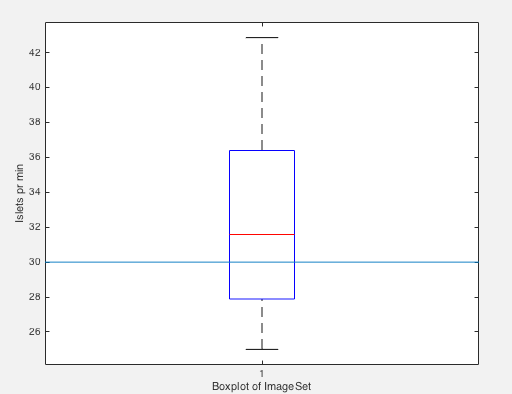
\includegraphics[width=0.5\textwidth]{billeder/software/boxplot.png}
	\caption{Boxplot af distrubutionen af øer pr. minut}
	\label{fig:boxplot}
\end{figure}

Selve flowsimuleringen sker i et for loop. Først udvælges en tilfældig celle ved hjælp af randi (uniform fordelt random variable). I for loopet opdateres dens center position ud fra 2 variabler (newXPos og newYPos). X positionen springer med et fast interval for hver iteration (160 px). Inden for loopet fastsættes start positionen for cellen med randi, som giver et tal mellem 0 og 1200 px, som er højden på billedet. Herefter opdateres den nye Y position ved hjælp af randn (normal fordelt random variabel) med middelværdi sat til startpositionen og en standard afvigelse på 50 pixels. I figur \ref{fig:flowsim} er flow simulationen illustreret for de i alt 18 sekvenser, med en graf for hver celle. Det ses at cellen flytter sin Y position for hver iteration i for loopet.

\begin{figure}[H]
	\centering
	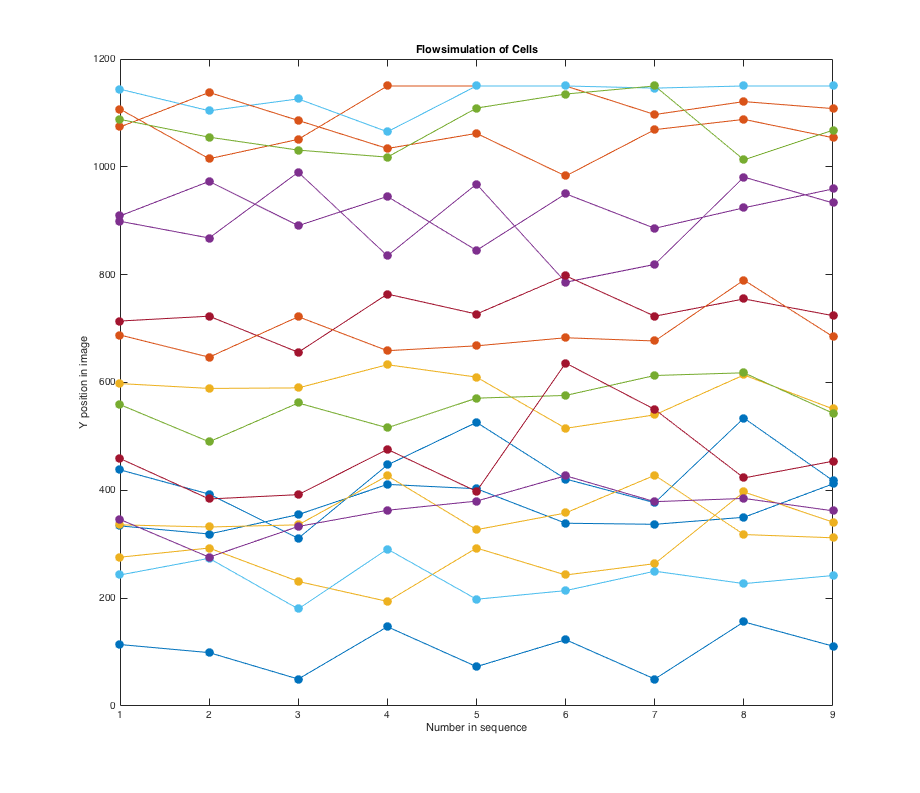
\includegraphics[width=0.5\textwidth]{billeder/software/Simulation.png}
	\caption{Illustration over flow simuleringen}
	\label{fig:flowsim}
\end{figure}

